\section{Visual Studio Projektmappe}

Das gesamte Projekt befindet sich in einer Visual Studio Projektmappe, welche in folgene Unterprojekte gegliedert ist:
\begin{itemize}
    \item \textbf{Common.Dal.Ado}:\newline Hier befinden sich Hilfsklassen, die den Umgang mit ADO.NET leichter gstalten.
    \item \textbf{Wetr.Domain}:\newline Dieses Projekt beinhaltet die Domainobjekte, welche als einfache Datenbehälter genutzt werden.
    \item \textbf{Wetr.BusinessLogic}:\newline Die Business Logik für \textit{Wetr.Simulator.Wpf} und \textit{Wetr.Cockpit.Wpf}. Beinhaltet die Anbindung an die benötigten \textit{ADO.NET} Implementierungen.
    \item \textbf{Wetr.BusinessLogic.Interface}:\newline Hier werden die Interfaces der einzelnen Manager definiert.
    \item \textbf{Wetr.Dal.Interface}:\newline In diesem Paket befinden sich die Interfaces für die Datenzugriffschricht für jedes Domainobjekt bzw. Tabelle.
    \item \textbf{Wetr.Dal.Ado}:\newline Die ADO.NET Implementierung der Datenzugriffsschicht Interfaces.
    \item \textbf{Wetr.Dal.Factory}:\newline Beinhaltet Factories um die Instanziierung der benötigen komkreten Klassen zu abstrahieren.
    \item \textbf{Wetr.Generator}: Zuständig für das Generieren von Messdaten für die einzelnen Stationen.
    \item \textbf{Wetr.Cockpit.Wpf}:\newline Cockpit Programm, verwendet WPF, MVVM Light Toolkit\footnote{http://www.mvvmlight.net}, MahAppsMetro\footnote{https://mahapps.com} und LiveCharts\footnote{https://lvcharts.net} um Usern die Möglichkeit zu geben Messtationen anzuzeigen bzw ändern zu können.
    \item \textbf{Wetr.Simulator.Wpf}:\newline Simulator Programm, verwendet ebenfalls WPF, MVVM Light Framework, MahAppsMetro und LiveCharts. Hier können Messwerte für Stationen generiert werden.
    \item \textbf{Wetr.Test.Dal}:\newline Dieses Projekt beinhaltet Unit-Tests für die Datenzugriffsschicht.
    \item \textbf{Wetr.Test.BusinessLogic}:\newline Dieses Projekt beinhaltet Unit-Tests für die BusinessLogic.
    \item \textbf{Wetr.Test.Web}\newline Projekt zum testen für die in \textbf{Wetr.Web} enthaltenen Funktionalitäten.
    \item \textbf{Wetr.Web} \newline Enthält alle notwendigen Funktionalitäten für einen REST-basierten Web-Service.
\end{itemize}

\newpage
\subsection{Common.Dal.Ado}
Das \textit{Common.Dal.Ado} Projekt verwendet die Klassen \textit{AdoTemplate}, \textit{DefaultConnectionFactory}, \textit{IConnectionFactory}, \textit{Parameter} und  \textit{RowMapper}. In der  \textit{AdoTemplate} Klasse werden alle anderen Klassen verwendet. Mithilfe  \textit{IConnection} wird eine Verbindung zu Datenbank aufgebaut.  \textit{AdoTemplate} stellt eine Funktion  \textit{QueryAsync} bereit um eine Datenbankabfragen durchführen zu können.

\begin{figure}[H]
\centering
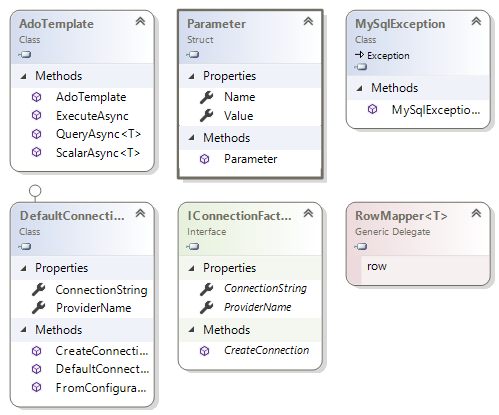
\includegraphics[width=.8\textwidth]{pictures/Common_Dal_Ado_ClassDiagramm.png}
\caption{Common.Dal.Ado UML Diagramm}
\label{fig:common.dal.ado}
\end{figure}
\raggedright

\newpage
\subsection{Wetr.BusinessLogic.Interface}
Das \textit{Wetr.BusinessLogic.Interface} Projekt definiert die Schnittstellen für die Manager in dem \textit{Wetr.BusinessLogic} Projekt.

\begin{figure}[H]
\centering
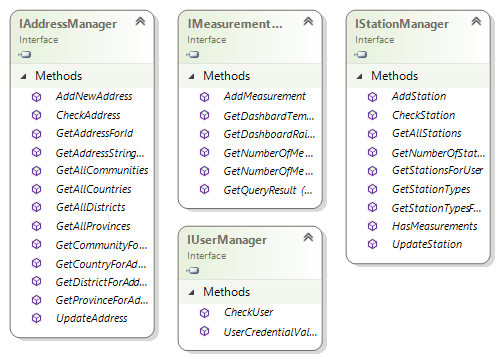
\includegraphics[width=\textwidth]{pictures/BusinessLogic_Interface.png}
\caption{Wetr.BusinessLogic.Interface UML Diagramm}
\label{fig:Wetr.BusinessLogic}
\end{figure}
\raggedright

\newpage
\subsection{Wetr.BusinessLogic}
Das \textit{Wetr.BusinessLogic} Projekt verwendet die \textit{Wetr.Dal.Factory} um die benötigten \textit{DAOs} zu erstellen. Die Business Logik stellt einen \textit{ManagerLocator} zu Verfügung der Instanzen der einzelnen Manager liefern kann. Jeder Manager stellt Funktionen zur Verfügung mit der Abfragen auf die Datenbank durchgeführt werden können.

\begin{figure}[H]
\centering
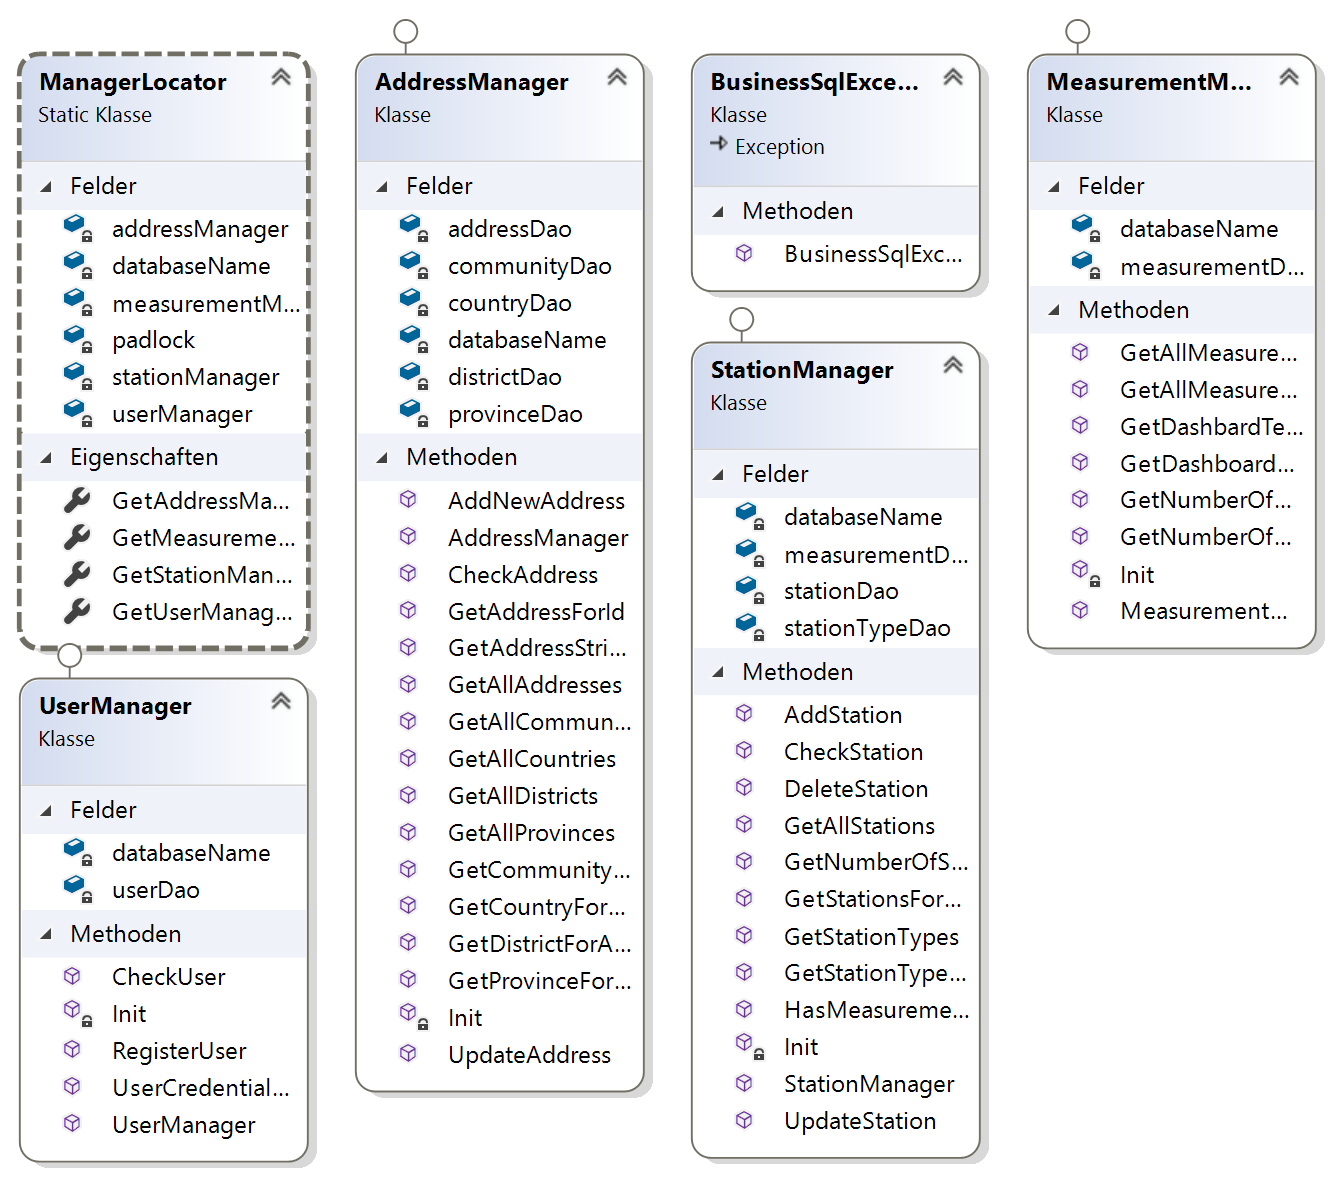
\includegraphics[width=\textwidth]{pictures/BusinessLogic.png}
\caption{Wetr.BusinessLogic UML Diagramm}
\label{fig:Wetr.BusinessLogic}
\end{figure}
\raggedright

\newpage
\subsection{Wetr.Dal.Interface}
Im \textit{Wetr.Dal.Interface} Projekt wird für jede Klasse in  \textit{Wetr.Domain} ein eigenes Interface bereitgestellt das von den jeweiligen \textit{Dao} Objekten implementiert wird. Jedes Interface implementiert \textit{IDaoBase}$<$\textit{T}$>$. Dieses Interface fasst die Methoden, die in jedem abgeleiteten \textit{Dao Objekt} implementiert werden müssen, zusammen (FindAll, FindById, Delete, Insert, Update).

\begin{figure}[H]
\centering
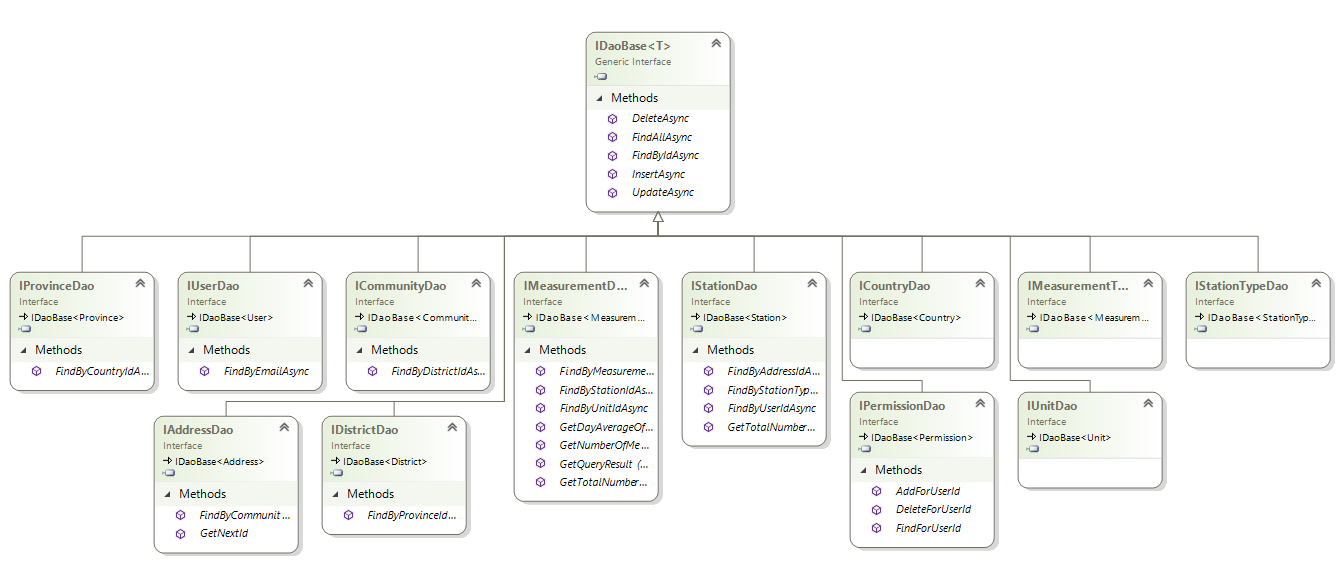
\includegraphics[width=\textwidth]{pictures/Wetr_Dal_Interface.png}
\caption{Wetr.Dal.Interface UML Diagramm}
\label{fig:Wetr.Dal.Interface}
\end{figure}
\raggedright

\newpage
\subsection{Wetr.Dal.Ado}
Mit den Klassen im \textit{Wetr.Dal.Ado} Projekt kann eine Verbindung zur Datenbank aufgebaut werden und spezielle SQL Operationen ausgeführt werden. Für jedes \textit{Dao} Objekt gibt es eine \textit{Wetr.Domänen} Klasse. Diese Klassen werden als Behälter Klassen für die angefragten Daten der Datenbank verwendet.

\begin{figure}[H]
\centering
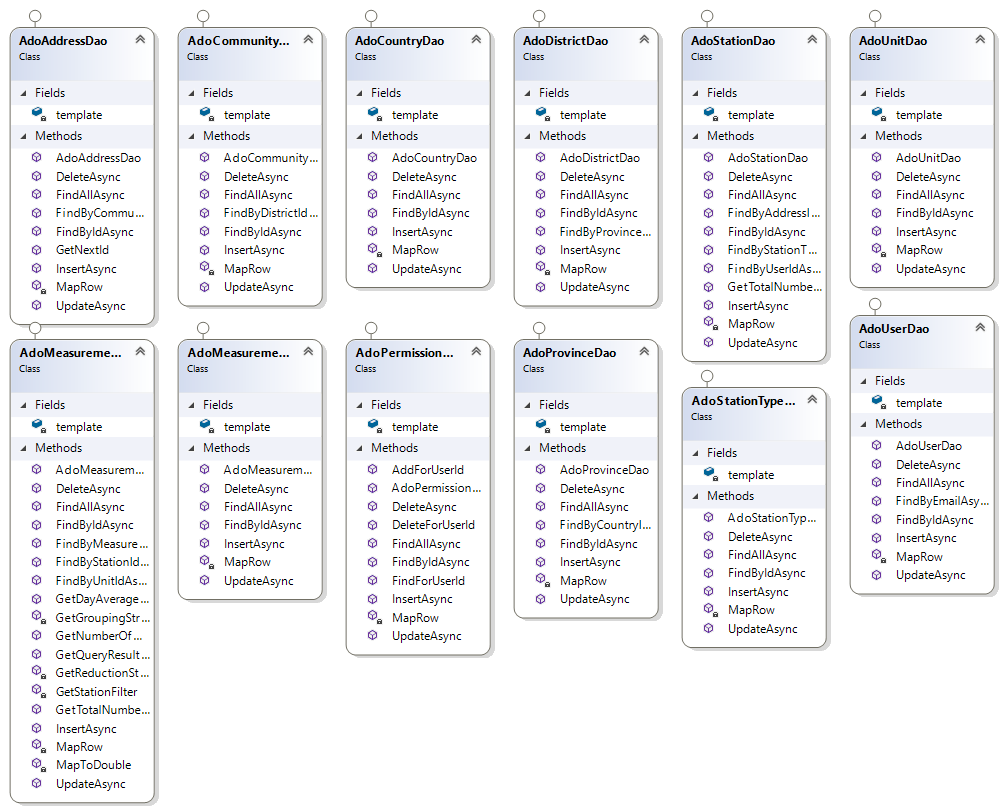
\includegraphics[width=\textwidth]{pictures/Wetr_Dal_Ado.png}
\caption{Wetr.Dal.Ado UML Diagramm}
\label{fig:Wetr.Dal.Ado}
\end{figure}
\raggedright

\newpage
\subsection{Wetr.Dal.Factory}
Im \textit{Wetr.Dal.Factory} Projekt wird eine Klasse \textit{AdoFactory} bereitgestellt mit deren Hilfe ein \textit{Dao} Objekt erstellt werden kann.

\begin{figure}[H]
\centering
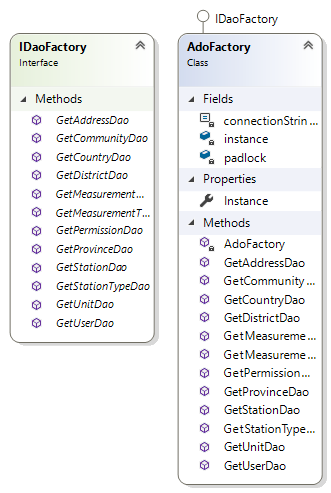
\includegraphics[width=.6\textwidth]{pictures/Wetr_Dal_Factory.png}
\caption{Wetr.Dal.Factory UML Diagramm}
\label{fig:Wetr.Dal.Factory}
\end{figure}
\raggedright

\newpage
\subsection{Wetr.Domain}
Das \textit{Wetr.Domain} Projekt enthält alle Behälterklassen für alle \textit{Dao} Objekte.

\begin{figure}[H]
\centering
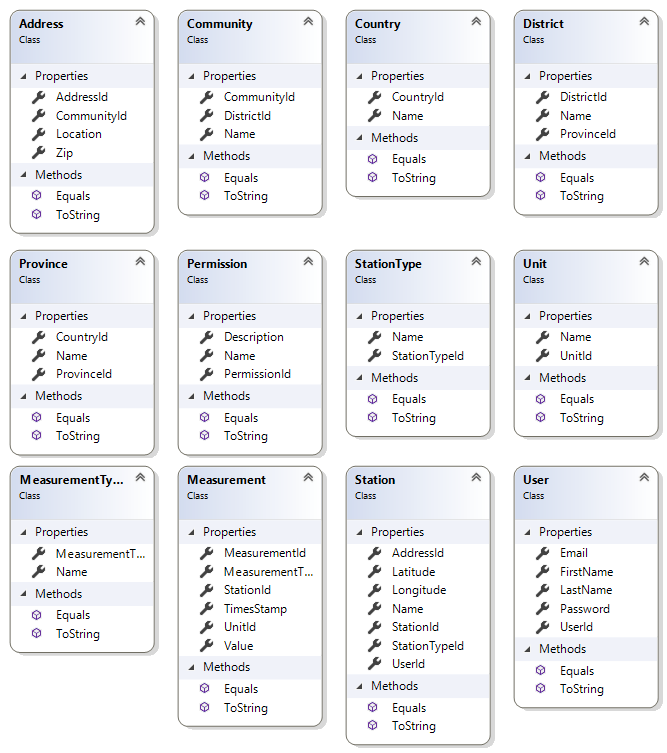
\includegraphics[width=.9\textwidth]{pictures/Wetr_Domain.png}
\caption{Wetr.Domain UML Diagramm}
\label{fig:Wetr.Domain}
\end{figure}
\raggedright

\newpage
\subsection{Wetr.Test.Dal}
Beim \textit{Wetr.Test.Dal} Projekt werden alle Funktionen von jedem \textit{Dao} Objekt getestet. Alle Tests wurden von der Klassen DaoBaseTest abgeleitet, welche Test für Dao-Methoden forcieren, welche in allen \textit{DAOs} implementiert wurden. 

\begin{figure}[H]
\centering
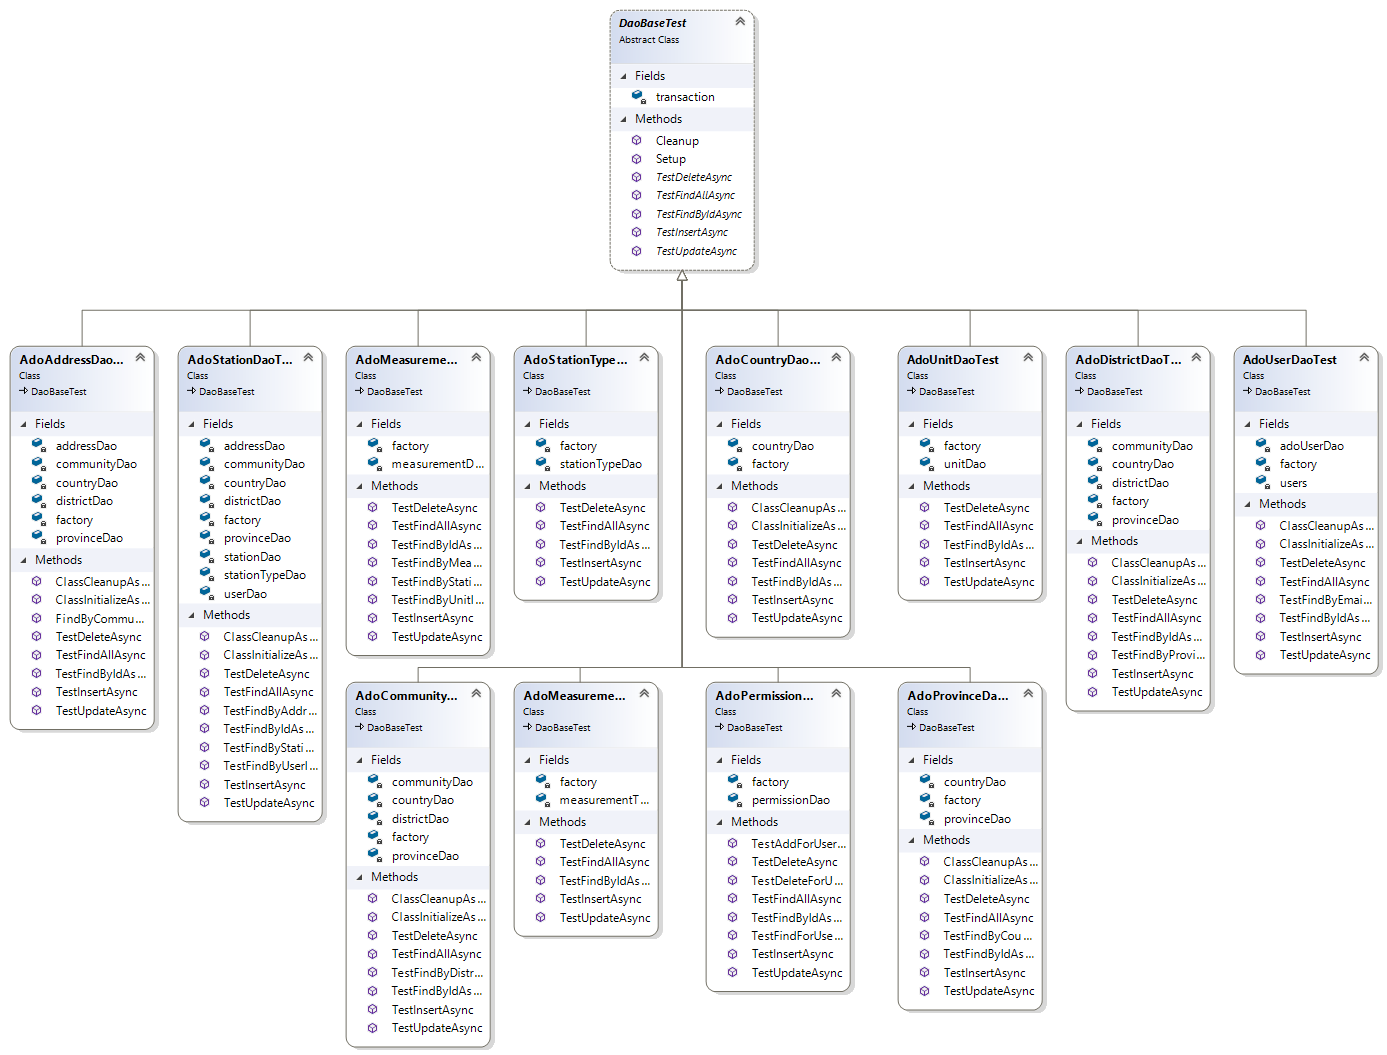
\includegraphics[width=\textwidth]{pictures/Wetr_Test_Dal.png}
\caption{Wetr.Test.Dal UML Diagramm}
\label{fig:Wetr.Test.Dal}
\end{figure}
\raggedright

\begin{figure}[H]
\centering
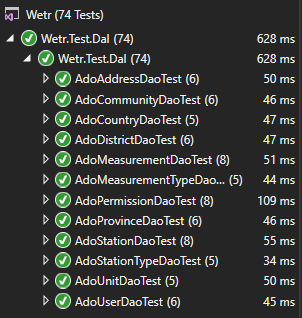
\includegraphics[width=.4\textwidth]{pictures/green_tests.png}
\caption{Beweis, dass die UnitTests erfolgreich durchlaufen.}
\label{fig:Wetr.Test.Dal}
\end{figure}
\raggedright

\newpage
\subsection{Wetr.Test.BusinessLogic}
Beim \textit{Wetr.Test.BusinessLogic} Projekt werden alle Funktionen der einzelnen Manager des \textit{Wetr.BusinessLogic} Projekts getestet.

\begin{figure}[H]
\centering
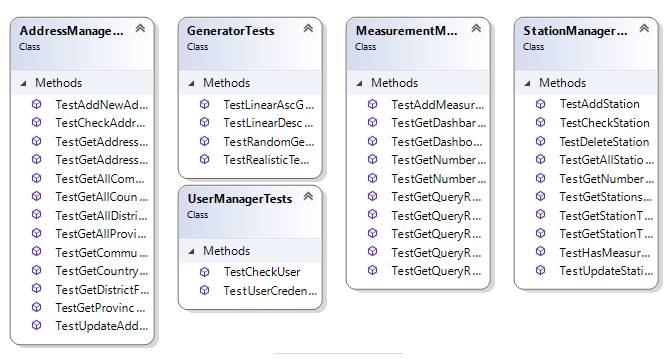
\includegraphics[width=\textwidth]{pictures/Wetr_Test_BusinessLogic.png}
\caption{Wetr.Test.BusinessLogic UML Diagramm}
\label{fig:Wetr.Test.Dal}
\end{figure}
\raggedright

\begin{figure}[H]
\centering
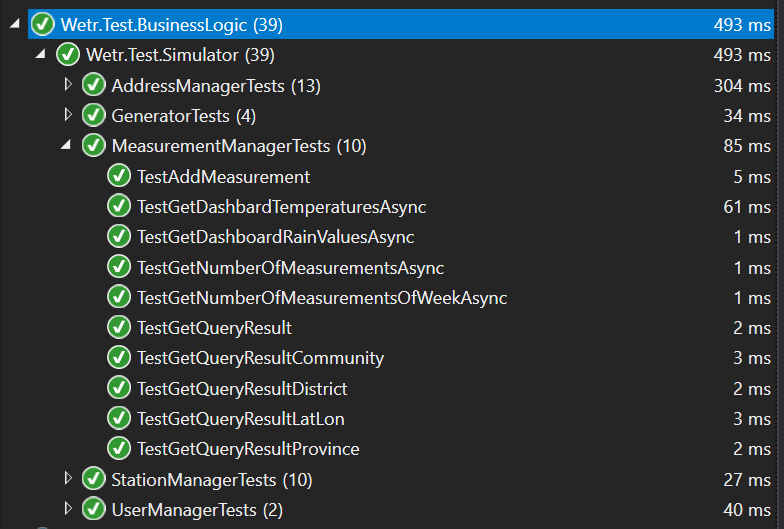
\includegraphics[width=0.8\textwidth]{pictures/bl_tests.png}
\caption{Beweis, dass die BusinessLogic UnitTests durchlaufen.}
\end{figure}
\raggedright

\newpage
\subsection{Wetr.Generator}
\label{sec:generator}

Der Generator generiert pro \textit{MeasurementType} eine eigene Datei, in der sich die generierten Messdaten befinden. Pro Typ werden nicht genau gleich viele Messdaten generiert, somit ergibt sich eine Summe von etwa 1.2 Millionen Messdaten. Das Format der erzeugten Dateien ist so gestaltet, damit es mit einem speziellen SQL Befehl mittels Bulk-Insert\footnote{https://dev.mysql.com/doc/refman/8.0/en/load-data.html} sehr schnell in die Datenbank aufgenommen werden kann. Die generierten Daten haben einen Zeitstempel, der sich innerhalb von einem Jahr bewegt.~\\~\\ %WTF LaTeX?

\textbf{Temperatur}\\
Es wird jede Stunde ein Messwert generiert, der je nach Jahreszeit die Temperatur nach natürlichem Verlauf, sprich zur Mittagszeit ist es am wärmste und in der Nacht am kältesten, gestaltet. Die Werte beinhalten eine zufällige Abweichung von $\pm 1.25$. Der Minimal- bzw. Maximalwert wird pro Jahreszeit nach klimatabelle.info festgelegt.~\\~\\ %WTF LaTeX?

\textbf{Luftfeuchtigkeit}\\
Die Berechnung der Luftfeuchtigkeit funktioniert gleich, wie die der Temperatur, nur, dass die durchschnittlichen Luftfeuchtigkeitswerte hergenommen wurden. Als zufällige Abweichung wurden $\pm10\%$ gewählt.~\\~\\ %WTF LaTeX?

\textbf{Niederschlag}\\
Da nur der jährliche Durchschnittsniederschlag pro Jahreszeit zur Verfügung stand, wurden nicht stündlich, sondern täglich ein Messert generiert. Dieser Wert bewegt sich zwischen $0$ und der Anzahl des durchschnittlichen Tagesniederschalag Mal zwei.~\\~\\ %WTF LaTeX?

\textbf{Luftdruck}\\
Jede Stunde wird ein Luftdruckwert generiert, der zufällig zwischen $900$ und $1100$ Hektopascal liegt.~\\~\\ %WTF LaTeX?

\textbf{Windrichtung}\\
Die Windrichtung ändert sich in dieser einfachen Simulation jede Stunde und kann von $0$ bis $360$ Grad betragen.~\\~\\ %WTF LaTeX?

\textbf{Windstärke}\\
Die Generierung der Windstärke ist in der aktuellen Ausbaustufe sehr primitiv gehalten und ändert sich stündlich zufällig von $0$ und $20\ km/h$.


\newpage
\subsection{Wetr.Cockpit.Wpf}
Das \textit{Wetr.Cockpit.Wpf} Projekt wird nach dem MVVM Prinzip\footnote{https://docs.microsoft.com/en-us/xamarin/xamarin-forms/enterprise-application-patterns/mvvm} erstellt. Als UI Framework wird \textit{mahapps.metro}\footnote{https://mahapps.com/} verwendet.\textit{Views} und \textit{ViewModels} werden verwendet und mithilfe von \textit{DataBinding} wird vom \textit{ViewModel} Daten bei der \textit{View} angezeigt. Nach dem erfolgreichen Login bietet das Cockpit Usern die Möglichkeit Messtationen zu editieren bzw hinzuzufügen. Im weiteren ist es dem User auch möglich die Messwerte seiner Stationen zu aggregieren.
\newline
\newline
Das Hauptprogramm (nach dem Login) ist in drei verschiedenen Tabs eingeteilt: \newline\textit{Home}, \textit{Analysis} und \textit{Stations}.
\newline
\newline
\textbf{Login}\newline
Beim Login wird in der Datenbank abgefragt ob der User mit der Email und dem Passwort in der Datenbank vorhanden ist. Das Passwort wird mithilfe von BCrypt.Net\footnote{https://www.nuget.org/packages/BCrypt.Net} auf Gültigkeit überprüft. \newline\newline
Ein Standard Benutzer:\newline
\textbf{Email}: test@test.com\newline
\textbf{Passwort}: 1234

\begin{figure}[H]
\centering
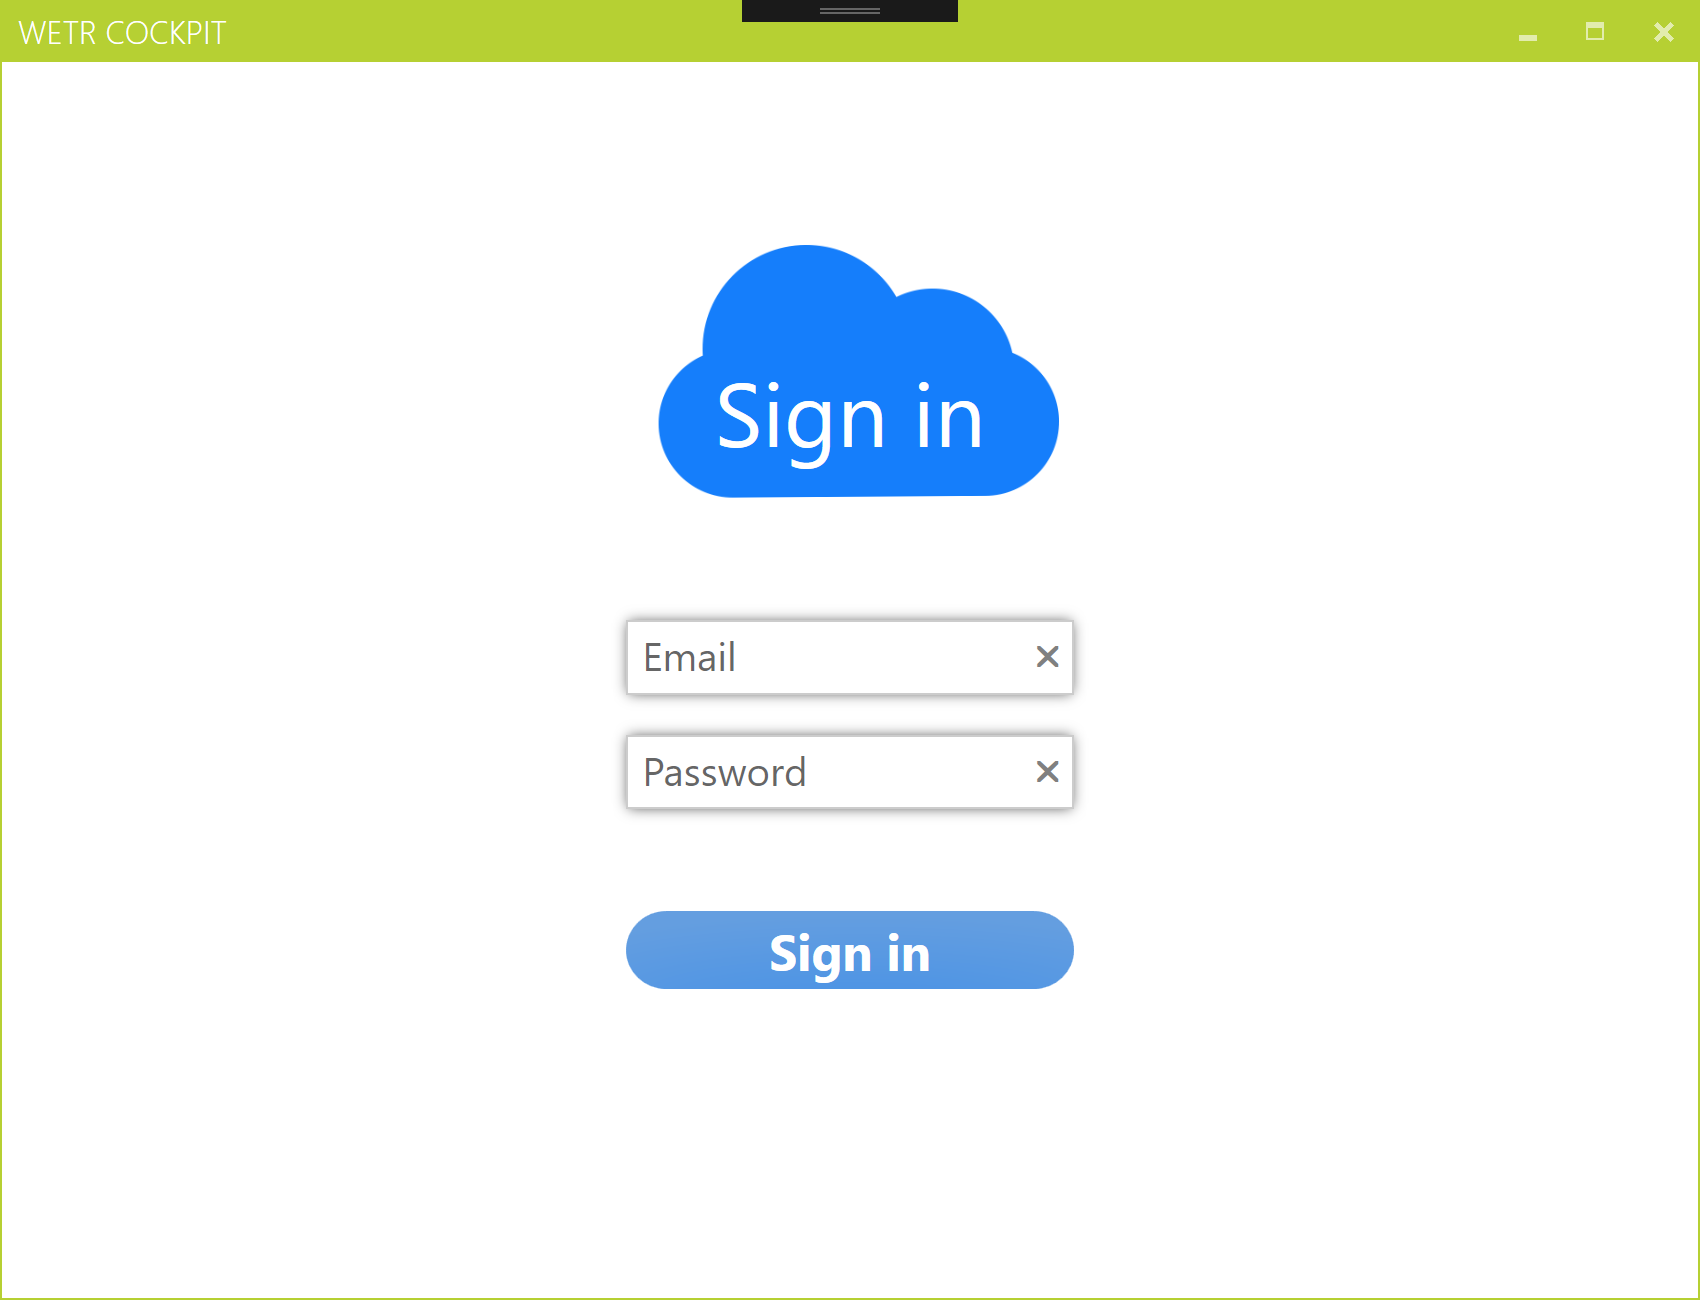
\includegraphics[width=.7\textwidth]{pictures/Cockpit/Cockpit_1.png}
\caption{Login View}
\label{fig:Wetr.Cockpit.Wpf.LoginView}
\end{figure}
\raggedright

\newpage
\textbf{Home}\newline
Eine kleine Übersicht über die Stationen des Users. Hier werden nützliche Werte für den User angezeigt (zb. Stationen Anzahl).

\begin{figure}[H]
\centering
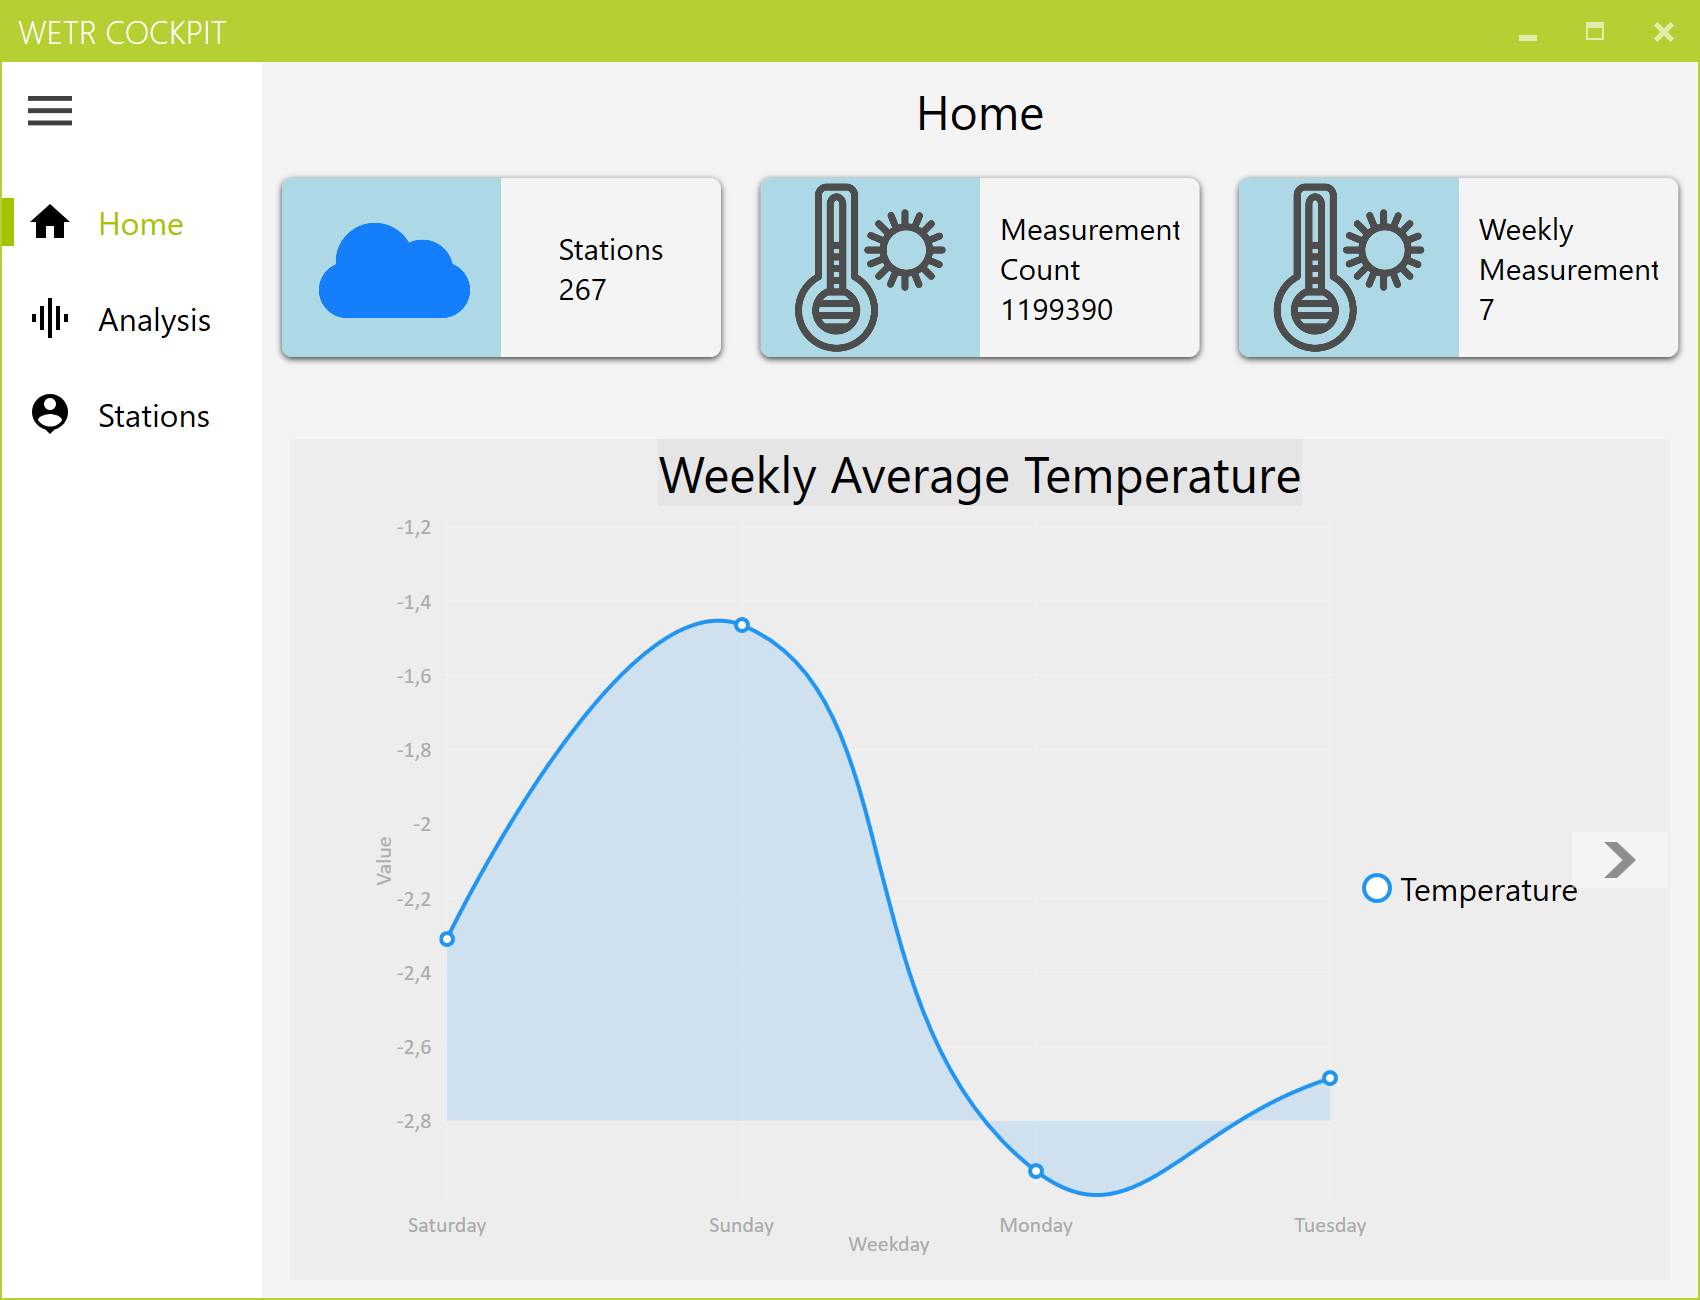
\includegraphics[width=.7\textwidth]{pictures/Cockpit/Cockpit_2.png}
\caption{Home View}
\label{fig:Wetr.Cockpit.Wpf.HomeView}
\end{figure}
\raggedright

\textbf{Analysis}\newline
Hier wird die Aggregation der Messwerte der Stationen ermöglicht. Einzelne Stationen und verschiedene Messwertarten können zum Aggregieren ausgewählt werden.

\begin{figure}[H]
\centering
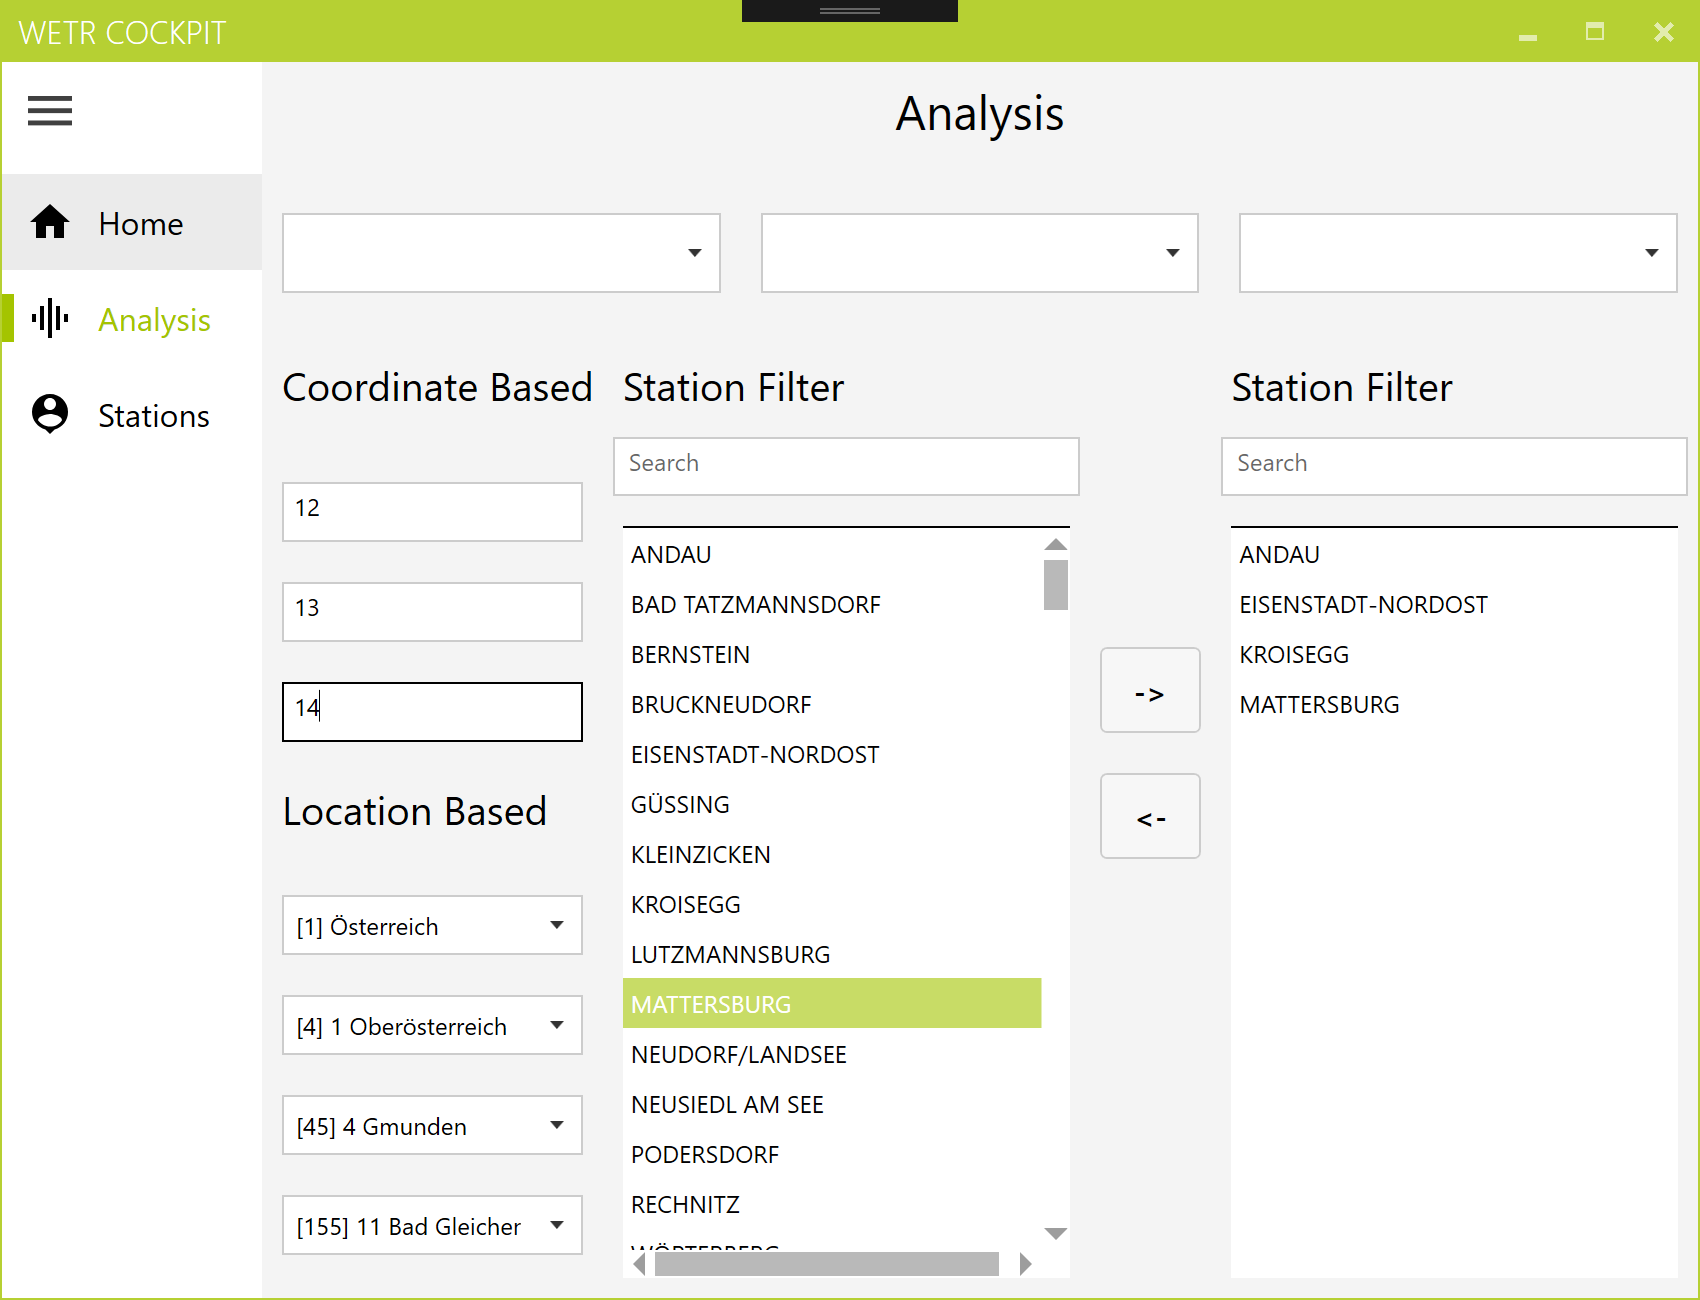
\includegraphics[width=.7\textwidth]{pictures/Cockpit/Cockpit_3.png}
\caption{Analysis View}
\label{fig:Wetr.Cockpit.Wpf.Analysis}
\end{figure}
\raggedright

\begin{figure}[H]
\centering
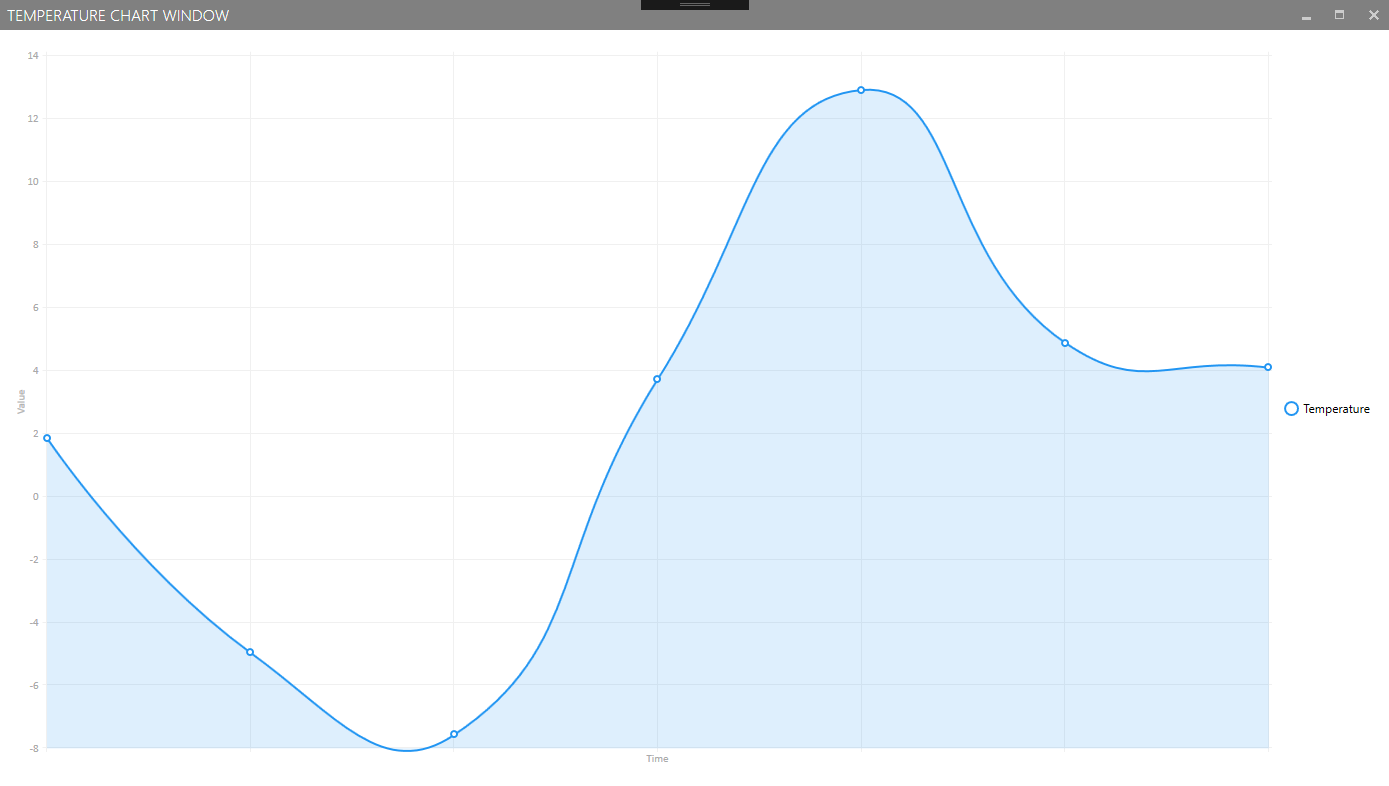
\includegraphics[width=.7\textwidth]{pictures/Cockpit/Cockpit_3_1.png}
\caption{Analysis View Aggregate Window}
\label{fig:Wetr.Cockpit.Wpf.Analysis2}
\end{figure}
\raggedright

\textbf{Stations}\newline
Im Tab Stations wird dem User die Möglichkeit geboten seine Stationen zu ändern oder neue Stationen hinzuzufügen.

\begin{figure}[H]
\centering
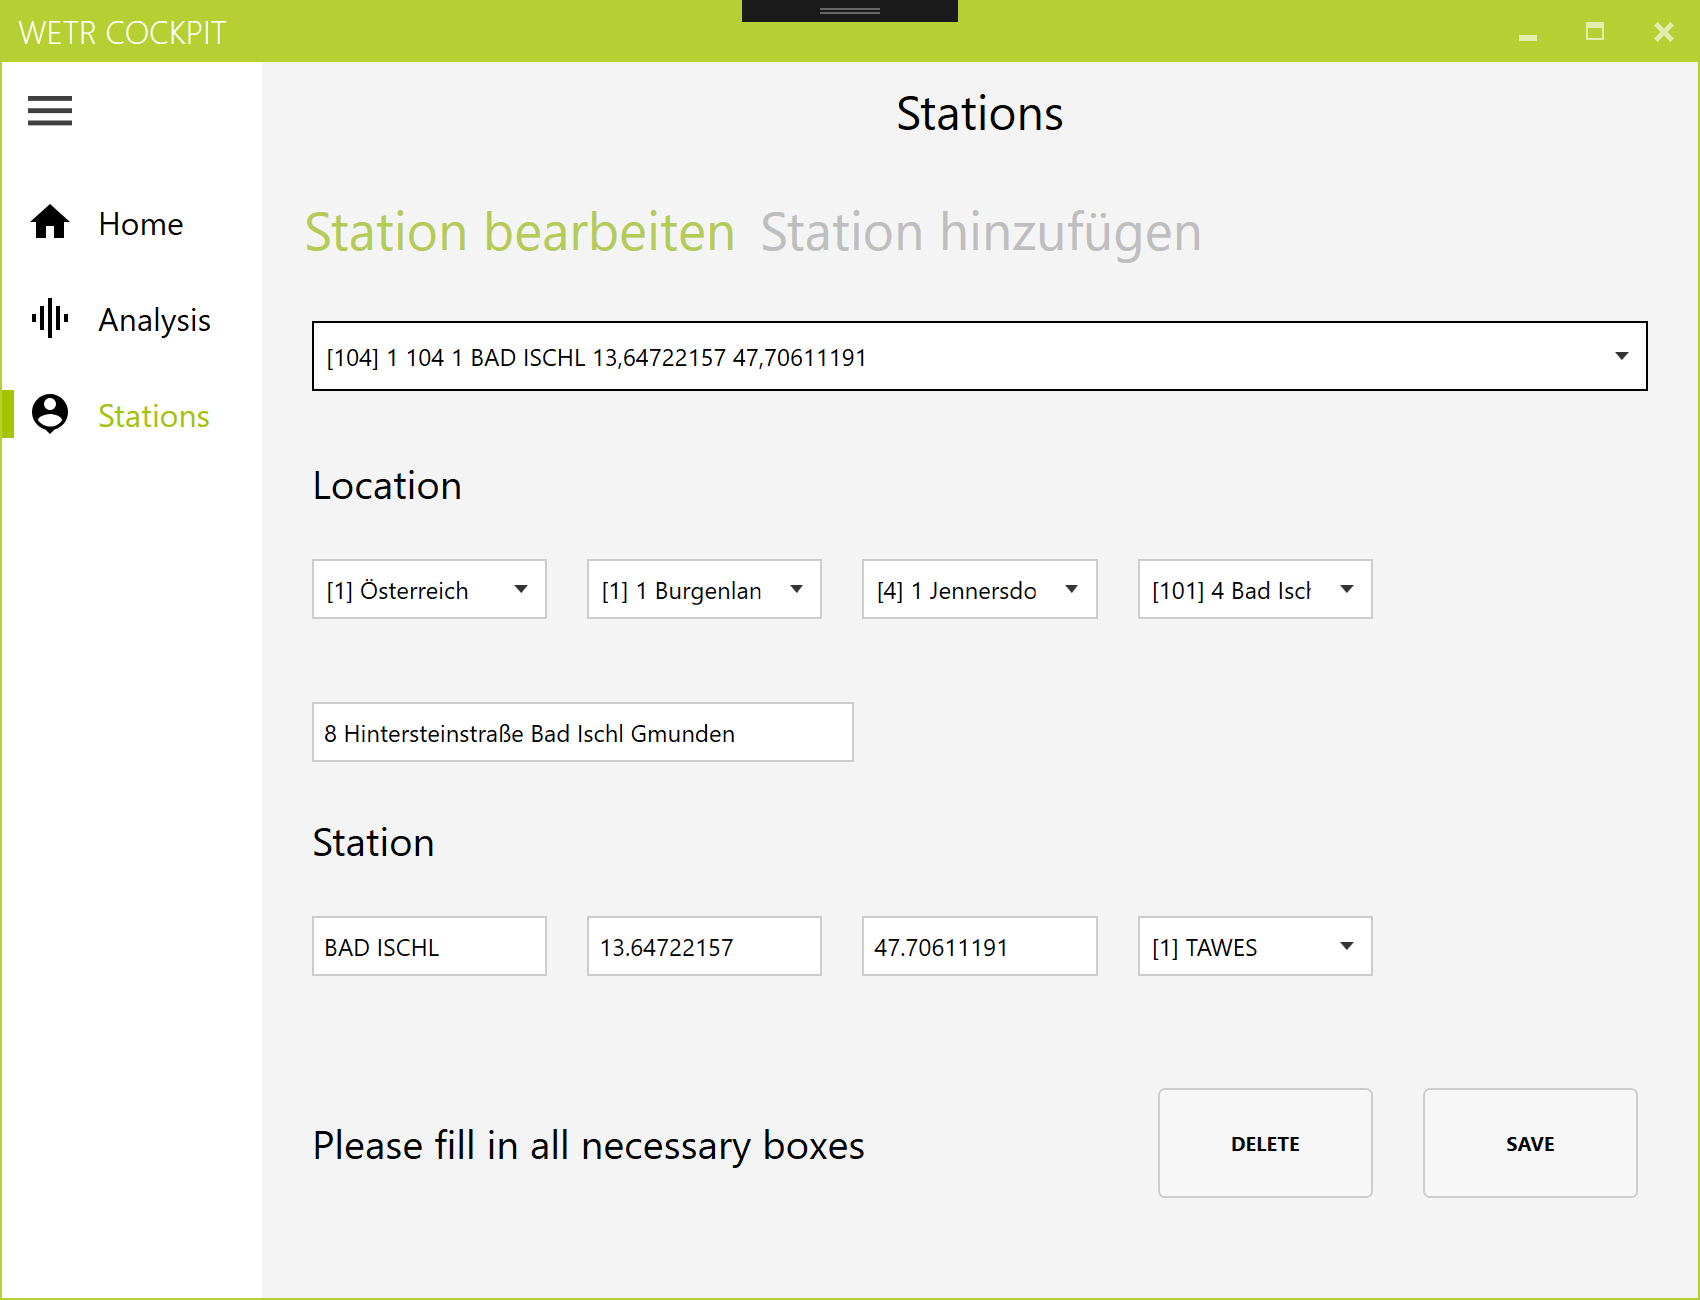
\includegraphics[width=.7\textwidth]{pictures/Cockpit/Cockpit_4.png}
\caption{Stations Edit View}
\label{fig:Wetr.Cockpit.Wpf.Station.Edit}
\end{figure}
\raggedright

\begin{figure}[H]
\centering
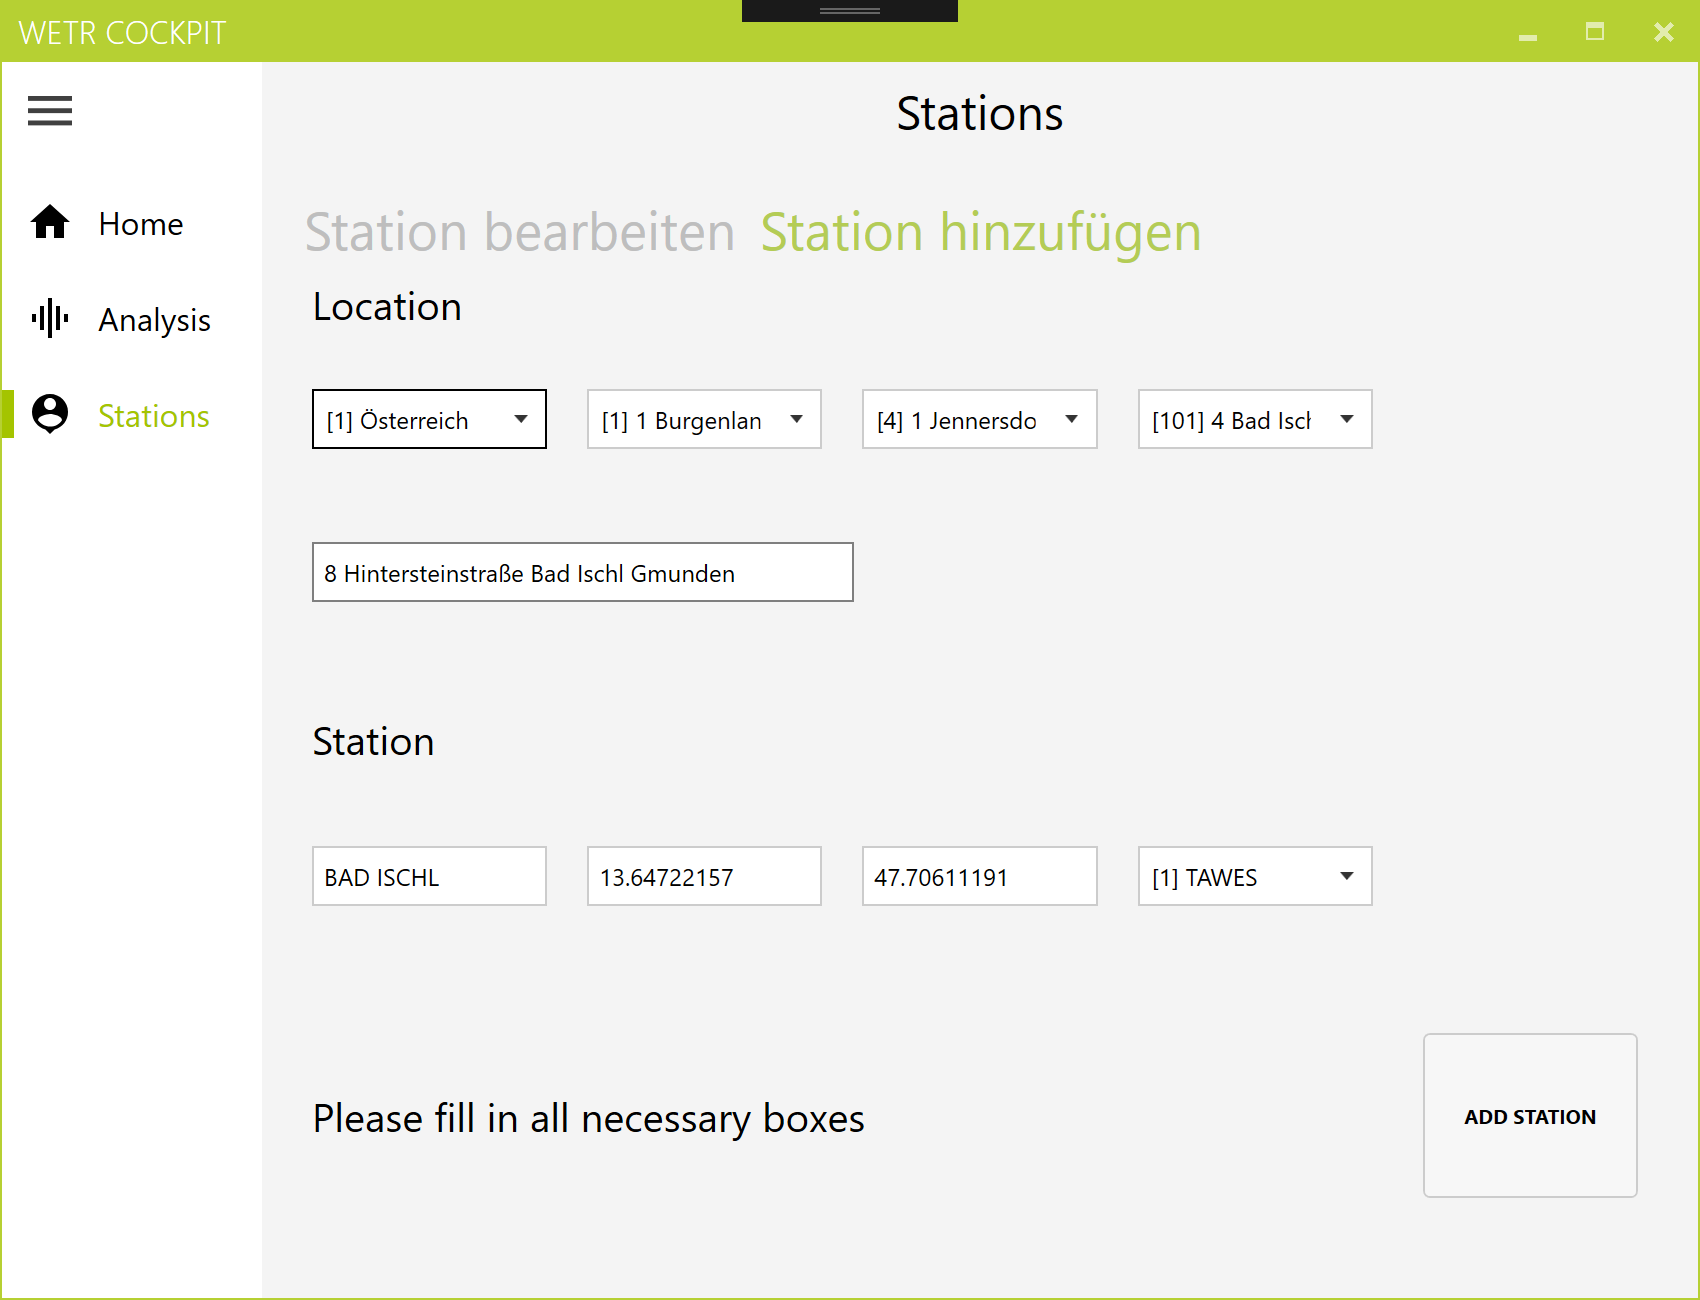
\includegraphics[width=.7\textwidth]{pictures/Cockpit/Cockpit_5.png}
\caption{Stations Add View}
\label{fig:Wetr.Cockpit.Wpf.Station.Add}
\end{figure}
\raggedright

\newpage
\subsection{Wetr.Simulator.Wpf}
Auch dieses Projekt wurde nach dem MVVM Prinzip erstellt. Als UI Framework wird \textit{mahapps.metro}\footnote{https://mahapps.com/} verwendet.
Der Simulator ist in 4 verschieden Bereiche unterteilt: \textit{Station selection}, \textit{Preset creation}, \textit{Preset assignment} und \textit{Simulation}. 
\newline
\newline
\textbf{Station selection}\newline
In diesem Bereich werden die Stationen ausgewählt die für die nachfolgenden Schritte verwendet werden.

\begin{figure}[H]
\centering
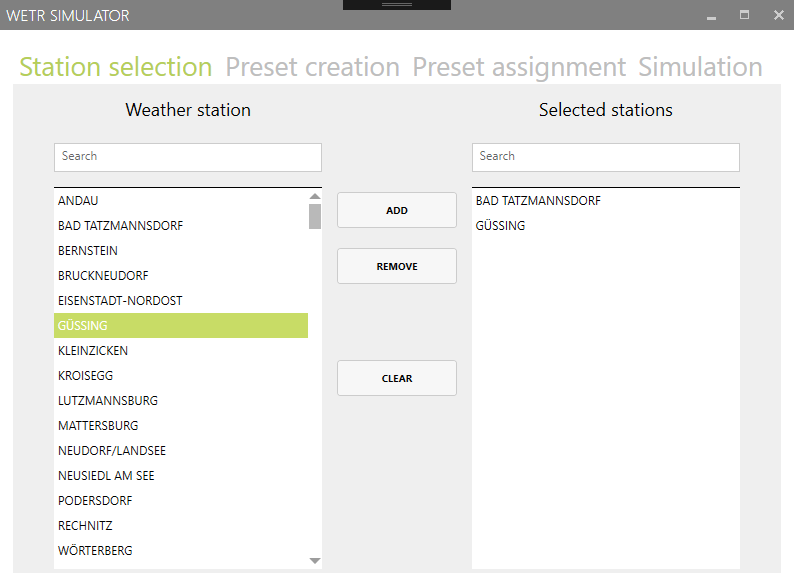
\includegraphics[width=.7\textwidth]{pictures/Simulator/Simulator_1_StationSelection.png}
\caption{Station selection}
\label{fig:Wetr.Simulator.Wpf.StationSelection}
\end{figure}
\raggedright

\newpage
\textbf{Preset creation}\newline
Ein \textit{Preset} ist eine Berechnungseinstellung. Für diese Einstellung können Daten wie Messart, Start und Enddatum, Minimum und Maximum der Berechnung, Berechnungsart (zb. Linear) und die Regelmäßigkeit der Berechnung eingestellt werden. 
Grundsätzlich können mehrere \textit{Presets} erstellt werden. Diese werden durch den vergebenen Namen identifiziert.

\begin{figure}[H]
\centering
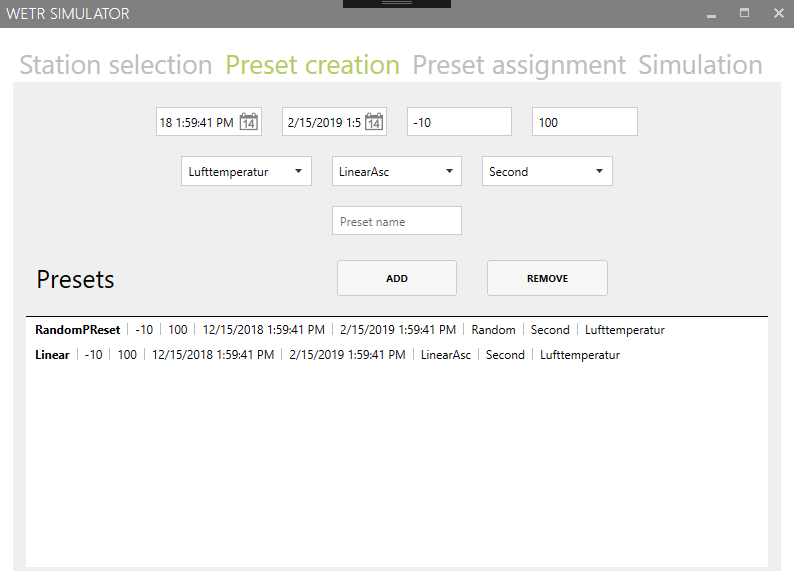
\includegraphics[width=.7\textwidth]{pictures/Simulator/Simulator_2_PresetCreation.png}
\caption{Preset creation}
\label{fig:Wetr.Simulator.Wpf.PresetCreation}
\end{figure}
\raggedright

\textbf{Preset assignment}\newline
Nachdem ein \textit{Preset} erstellt wurde kann diesem eine \textit{Station} zugeteilt werden. Nur \textit{Stationen} die am Anfang ausgewählt wurden können hinzugefügt werden.

\begin{figure}[H]
\centering
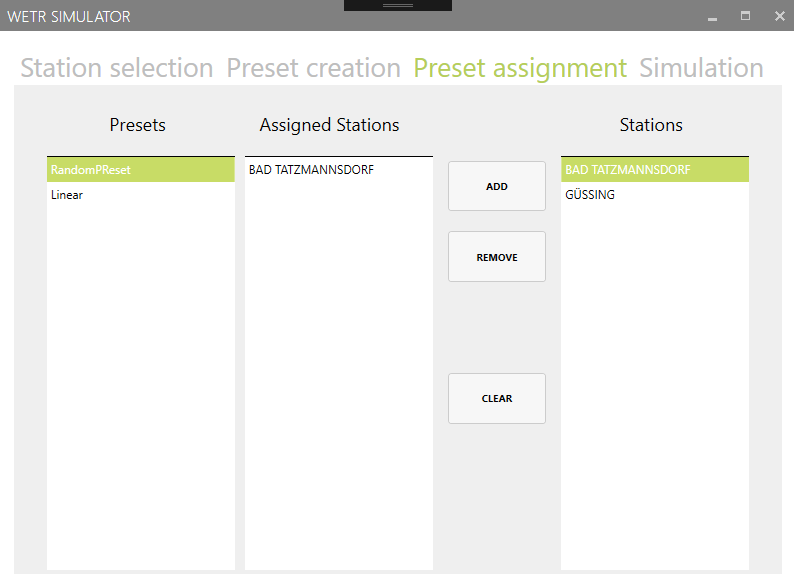
\includegraphics[width=.7\textwidth]{pictures/Simulator/Simulator_3_PresetAssignment.png}
\caption{Preset assignment}
\label{fig:Wetr.Simulator.Wpf.PresetAssignment}
\end{figure}
\raggedright

\textbf{Simulation}\newline
In diesem Bereich können nun die zuvor erstellen \textit{Presets} simuliert werden. Durch auswählen eines \textit{Presets} und anschließendem Starten der Simulation können die Zwischenergebnisse in dem Graphen daneben angezeigt werden. 
Falls die Geschwindigkeit einer Simulation zu langsam ist kann diese mit dem Schieber über dem Graphen verändert werden.

\begin{figure}[H]
\centering
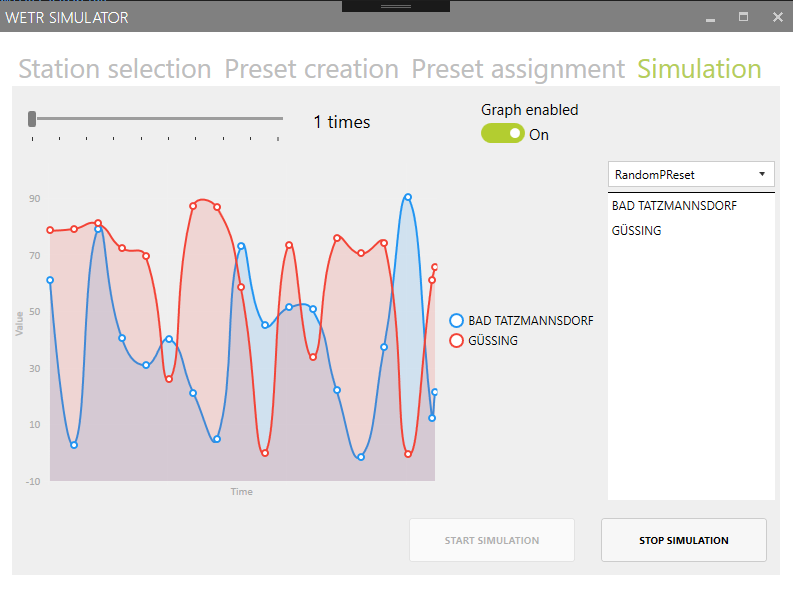
\includegraphics[width=.7\textwidth]{pictures/Simulator/Simulator_4_Simulation.png}
\caption{Simulation}
\label{fig:Wetr.Simulator.Wpf.Simulation}
\end{figure}
\raggedright

\newpage

\subsection{Wetr.Web}
Siehe Abschnitt \ref{rest}.

\begin{figure}[H]
\centering
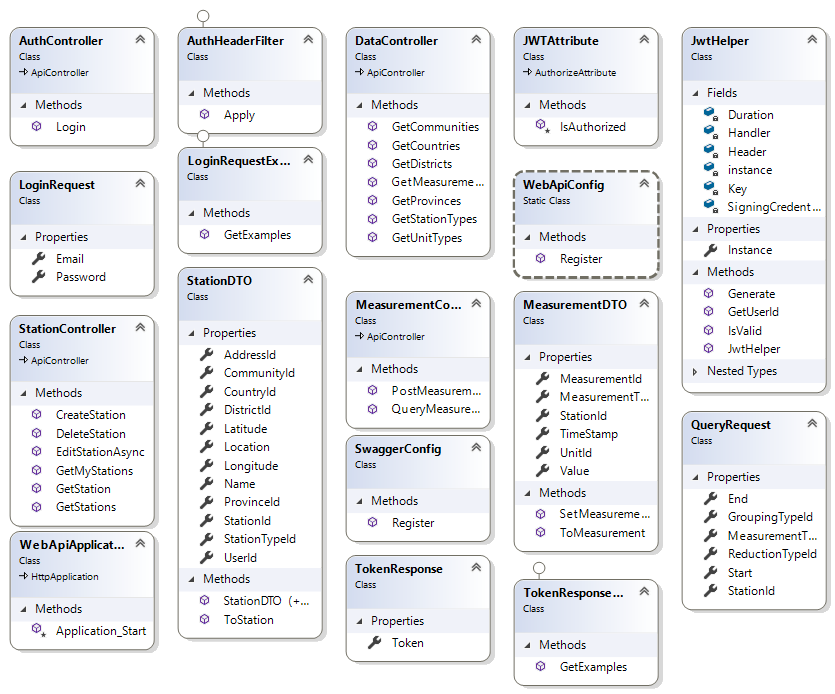
\includegraphics[width=\textwidth]{pictures/Wetr_Web.png}
\caption{Wetr.Web UML}
\label{fig:Wetr.Web.UML}
\end{figure}
\raggedright

\subsection{Wetr.Test.Web}
Für dieses Projekt wurden Test für die JavaWebToken-Authentifizierung geschrieben.


\begin{figure}[H]
\centering
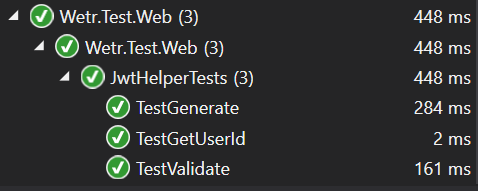
\includegraphics[width=.5\textwidth]{pictures/webtest.PNG}
\caption{Durchlaufende UnitTests}
\end{figure}
\raggedright
\subsection{Wetr.ApiManager}
Der \textit{Wetr.ApiManager} wird vom \textit{Wetr.Simulator} verwendet um Stationen zu laden und Measurement Daten in der Datenbank mithilfe der Rest Schnittstelle zu speichern. Der \textit{Wetr.ApiManager} stellt zwei Funktionen, \textit{GetStations} und \textit{PostMeasurement} zur Verfügung die mithilfe eines \textit{HttpClient} einen \textit{Get} bzw. \textit{Post request} senden.

\newpage